% !TeX root = ../../../main.tex
\subsection{Sensitivity of Event Matching Threshold}
\label{ch06:apd:threshold_sweep}

Event matching is performed using cosine distance between PubMedBERT embeddings with threshold $\theta = 0.10$ (Section~\ref{ch06:sec:evaluation_methodology_metrics}).
Because the event match rate depends directly on $\theta$, we conducted a sensitivity analysis by sweeping $\theta$ from $0.01$ to $0.50$ in increments of $0.01$ and recomputing match rate, concordance, and AULTC for each model.


% !TeX root = ../../../main.tex
\begin{figure}[htbp]
\begin{ChSixFloatBody}

    \centering
    \begin{minipage}[t]{0.48\columnwidth}
        \centering
        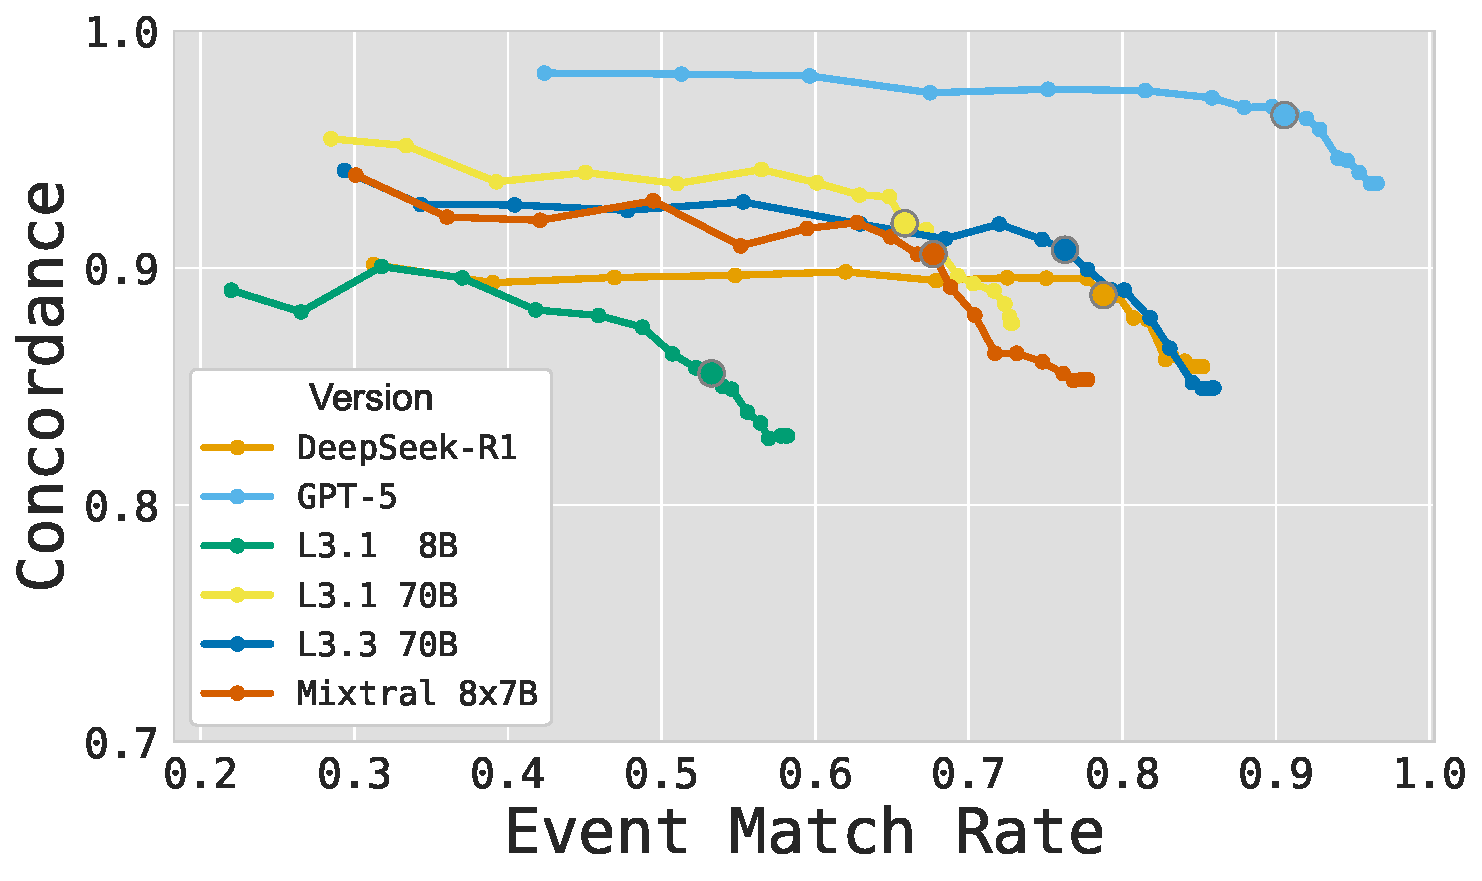
\includegraphics[width=\linewidth]{Appendices/appendix-ch06/images/figures/apd_figs/concordance_vs_event_match_rate.pdf}
        
    \end{minipage}\hfill
    \begin{minipage}[t]{0.48\columnwidth}
        \centering
        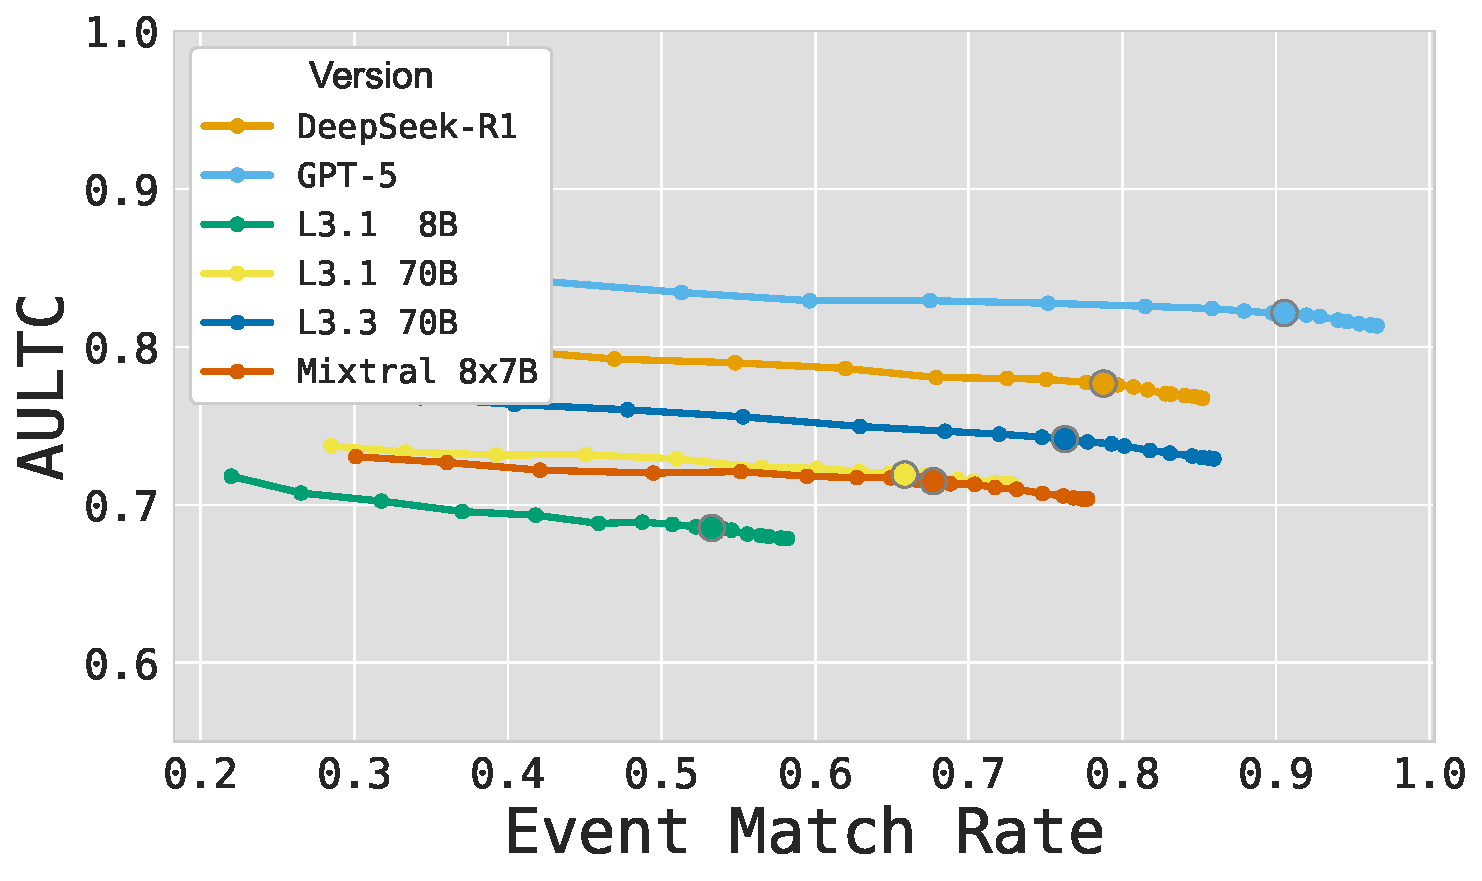
\includegraphics[width=\linewidth]{Appendices/appendix-ch06/images/figures/apd_figs/aultc_vs_event_match_rate.pdf}
    \end{minipage}
    
    

\end{ChSixFloatBody}
\caption{Sensitivity of temporal metrics to the cosine distance threshold $\theta$ for the recursive matching heuristic. Left: Concordance versus event match rate obtained by sweeping $\theta$ in increments of $0.01$ over $[0.01, 0.50]$. Right: AULTC versus event match rate under the same sweep. Each point ($\cdot$) corresponds to a distinct threshold value; the solid large circle ($\bullet$) denotes the threshold $\theta = 0.10$ used throughout the paper.}\ChSixFloatLabel{ch06:fig:threshold_sweep}
\ChSixUncaptionedPanelLabel{ch06:fig:threshold_sweep:concordance}
\ChSixUncaptionedPanelLabel{ch06:fig:threshold_sweep:aultc}
\end{figure}


Figure~\ref{ch06:fig:threshold_sweep} shows concordance and AULTC as functions of event match rate induced by varying $\theta$ on the \texttt{sepsis-40} dataset.
As expected, increasing $\theta$ monotonically increases event match rate.
However, beyond a moderate threshold, additional matches correspond to increasingly loose semantic alignments, which degrade temporal metrics.
This produces a characteristic trade-off curve: initial increases in match rate are accompanied by minimal degradation in concordance and AULTC, followed by a sharper decline once lower-quality matches are admitted.

Across models, we observe a clear ``elbow'' region near $\theta = 0.10$--$0.15$, where match rate increases modestly while concordance and AULTC remain stable. Beyond this region, particularly past $\theta \approx 0.20$, both concordance and AULTC begin to decline (with concordance drop being more rapid), indicating that additional matches are likely false positive alignments that impair temporal fidelity.

The threshold $\theta = 0.10$ used in the main analysis lies within this elbow region, balancing semantic precision and temporal robustness.
Importantly, relative model ordering remains stable across a wide range of thresholds, suggesting that conclusions regarding comparative performance are not artifacts of a particular cosine distance cutoff of the embeddings.
These results support the use of $\theta = 0.10$ as a conservative and temporally faithful operating point for event matching.





\FloatBarrier
